\documentclass[letter]{book}

\usepackage{graphics}
\begin{document}

Los documentos para \verb+lilypond-book+ pueden mezclar libremente
música y texto. Por ejemplo:

{%
\parindent 0pt
\noindent
\ifx\preLilyPondExample \undefined
\else
  \expandafter\preLilyPondExample
\fi
\def\lilypondbook{}%
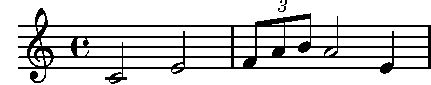
\includegraphics{./27/lily-bb6444e8-1}%
% eof

\ifx\postLilyPondExample \undefined
\else
  \expandafter\postLilyPondExample
\fi
}

Las opciones se escriben entre corchetes.

\begin{quote}
\noindent
\begin{verbatim}
    \language "espanol"
    do'4 fa16
\end{verbatim}
{%
\parindent 0pt
\noindent
\ifx\preLilyPondExample \undefined
\else
  \expandafter\preLilyPondExample
\fi
\def\lilypondbook{}%
\includegraphics{./fa/lily-e5cf3146-1}%
% eof

\ifx\postLilyPondExample \undefined
\else
  \expandafter\postLilyPondExample
\fi
}
\end{quote}

Los ejemplos grandes se pueden grabar en archivos separados e
introducirse con \verb+\lilypondfile+.

\begin{quote}
{%
\parindent 0pt
\noindent
\ifx\preLilyPondExample \undefined
\else
  \expandafter\preLilyPondExample
\fi
\def\lilypondbook{}%
\includegraphics{./6d/lily-dc72f8f6-1}%
\ifx\betweenLilyPondSystem \undefined
  \linebreak
\else
  \expandafter\betweenLilyPondSystem{1}%
\fi
\includegraphics{./6d/lily-dc72f8f6-2}%
\ifx\betweenLilyPondSystem \undefined
  \linebreak
\else
  \expandafter\betweenLilyPondSystem{2}%
\fi
\includegraphics{./6d/lily-dc72f8f6-3}%
\ifx\betweenLilyPondSystem \undefined
  \linebreak
\else
  \expandafter\betweenLilyPondSystem{3}%
\fi
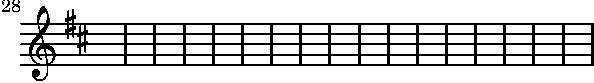
\includegraphics{./6d/lily-dc72f8f6-4}%
\ifx\betweenLilyPondSystem \undefined
  \linebreak
\else
  \expandafter\betweenLilyPondSystem{4}%
\fi
\includegraphics{./6d/lily-dc72f8f6-5}%
% eof

\ifx\postLilyPondExample \undefined
\else
  \expandafter\postLilyPondExample
\fi
}
\end{quote}

(Si es necesario, sustituya @file{screech-and-boink.ly}
por cualquier archivo @file{.ly}
situado en el mismo directorio que este archivo.)

\end{document}
